% !TeX program = xelatex
\documentclass[12pt,a4paper]{article}

% 基础包
\usepackage{amsmath,amssymb}
\usepackage{geometry}
\geometry{top=2.54cm, bottom=2.54cm, left=3.17cm, right=3.17cm}
\usepackage{booktabs}
\usepackage{array}
\usepackage{listings}
\usepackage{xcolor}
\usepackage{titlesec}
\usepackage{titletoc}
\usepackage{fancyhdr}
\usepackage{float}
\usepackage{setspace}
\usepackage{graphicx}
\usepackage{indentfirst}
\usepackage{algorithm}
\usepackage{algorithmicx}
\usepackage{algpseudocode}
\usepackage{tikz}
\usetikzlibrary{shapes,arrows,positioning}
\usepackage{subcaption}
\usepackage{multicol}
\usepackage{multirow}
\usepackage{tabularx}
\usepackage{makecell}
\usepackage{lastpage}
\usepackage{hyperref}
\usepackage{caption}
\usepackage[titles]{tocloft}

% 超链接设置
\hypersetup{
    hidelinks,
    colorlinks=false,
    pdfborder={0 0 0}
}

% 表格宽度设置
\newcolumntype{C}{>{\centering\arraybackslash}X}
\newcolumntype{L}{>{\raggedright\arraybackslash}X}
\newcolumntype{R}{>{\raggedleft\arraybackslash}X}

% Overleaf中文配置
\usepackage{xeCJK}
\setCJKmainfont{SimSun}[AutoFakeBold=4,AutoFakeSlant=0.15]    % 宋体风格
\setCJKsansfont{SimHei}[AutoFakeBold=4]     % 黑体风格
\setCJKmonofont{NSimSun}

% 英文主字体
\setmainfont{Times New Roman}

% ========== 字体字号设置（根据Word文档要求）==========
% 正文：宋体小四号（12pt），行距固定值24磅
\newcommand{\maintextfont}{\CJKfontspec{SimSun}[AutoFakeBold=4,AutoFakeSlant=0.15]\fontsize{12pt}{24pt}\selectfont}

% 一级标题：黑体小三号（15pt），行距固定值24磅
\newcommand{\sectionfont}{\CJKfontspec{SimHei}[AutoFakeBold=4]\fontsize{15pt}{24pt}\selectfont}

% 二级标题：楷体四号（14pt），行距固定值24磅
\newcommand{\subsectionfont}{\CJKfontspec{KaiTi}\fontsize{14pt}{24pt}\selectfont}

% 三级标题：宋体小四号加粗（12pt），行距固定值24磅
\newcommand{\subsubsectionfont}{\CJKfontspec{SimSun}[AutoFakeBold=4]\fontsize{12pt}{24pt}\selectfont}

% 四级标题：宋体小四号（12pt），行距固定值24磅
\newcommand{\paragraphfont}{\CJKfontspec{SimSun}[AutoFakeBold=4,AutoFakeSlant=0.15]\fontsize{12pt}{24pt}\selectfont}

% 摘要、目录、参考文献等名称：黑体四号（14pt），行距固定值24磅
\newcommand{\sectiontitlefont}{\CJKfontspec{SimHei}[AutoFakeBold=4]\fontsize{14pt}{24pt}\selectfont}

% 关键词名称：黑体小四号（12pt），行距固定值24磅
\newcommand{\keywordtitlefont}{\CJKfontspec{SimHei}[AutoFakeBold=4]\fontsize{12pt}{24pt}\selectfont}

% 表格标题：宋体小四号（12pt），行距固定值24磅
\newcommand{\tablecaptionfont}{\CJKfontspec{SimSun}[AutoFakeBold=4,AutoFakeSlant=0.15]\fontsize{12pt}{24pt}\selectfont}

% 图标题：宋体小四号（12pt），行距固定值24磅
\newcommand{\figurecaptionfont}{\CJKfontspec{SimSun}[AutoFakeBold=4,AutoFakeSlant=0.15]\fontsize{12pt}{24pt}\selectfont}
% ==================================================

% 行距设置：除表格外，全部固定值24磅
\setlength{\baselineskip}{24pt}
\renewcommand{\baselinestretch}{1}

% 正文使用主字体
\AtBeginDocument{\maintextfont}

% 正文首行缩进2字符
\setlength{\parindent}{2em}

% 页眉页脚设置
\pagestyle{fancy}
\fancyhf{}
\fancyfoot[C]{\thepage}
\renewcommand{\headrulewidth}{0pt}

% 章节标题格式
\titleformat{\section}{\centering\sectionfont}{\thesection}{1em}{}
\titleformat{\subsection}{\subsectionfont}{\thesubsection}{1em}{}
\titleformat{\subsubsection}{\subsubsectionfont}{\thesubsubsection}{1em}{}
\titleformat{\paragraph}{\paragraphfont}{\theparagraph}{1em}{}
\titleformat{\subparagraph}{\paragraphfont}{\thesubparagraph}{1em}{}

% 目录格式设置
\renewcommand{\cfttoctitlefont}{\hfill\sectiontitlefont}
\renewcommand{\cftaftertoctitle}{\hfill}
\renewcommand{\cftlottitlefont}{\hfill\sectiontitlefont}
\renewcommand{\cftafterlottitle}{\hfill}
\renewcommand{\cftloftitlefont}{\hfill\sectiontitlefont}
\renewcommand{\cftafterloftitle}{\hfill}
\renewcommand{\cftsecfont}{\maintextfont}
\renewcommand{\cftsubsecfont}{\maintextfont}
\renewcommand{\cftsubsubsecfont}{\maintextfont}

% 设置图表编号格式为中文（图1、表1）
\renewcommand{\thetable}{\arabic{table}}
\renewcommand{\thefigure}{\arabic{figure}}
\renewcommand{\tablename}{表}
\renewcommand{\figurename}{图}

% 设置表格清单和插图清单的标题
\renewcommand{\listtablename}{\centering\sectiontitlefont 表格清单}
\renewcommand{\listfigurename}{\centering\sectiontitlefont 插图清单}

% 摘要环境
\newenvironment{abstractcn}{%
    {\centering\sectiontitlefont 摘要\par}
    \par\maintextfont
}{%
    \par
}
\newenvironment{abstracten}{%
    {\centering\sectiontitlefont Abstract\par}
    \par\maintextfont
}{%
    \par
}

% 关键词命令
\newcommand{\keywords}[1]{\noindent{\keywordtitlefont 关键词：}\maintextfont #1}
\newcommand{\keywordsen}[1]{\noindent{\keywordtitlefont Keywords:}\maintextfont #1}

% 图表标题设置
\captionsetup[table]{
    labelsep=space,
    justification=centering,
    font={normalsize,rm},
    labelfont={normalsize,rm}
}
\captionsetup[figure]{
    labelsep=space,
    justification=centering,
    font={normalsize,rm},
    labelfont={normalsize,rm}
}

% 表格内容行距为单倍行距
\let\oldtabular\tabular
\let\oldendtabular\endtabular
\renewenvironment{tabular}[2][]{%
    \par\setlength{\baselineskip}{12pt}% 单倍行距
    \oldtabular[#1]{#2}%
}{%
    \oldendtabular
    \par\setlength{\baselineskip}{24pt}% 恢复24磅
}

\let\oldtabularx\tabularx
\let\oldendtabularx\endtabularx
\renewenvironment{tabularx}[2]{%
    \par\setlength{\baselineskip}{12pt}% 单倍行距
    \oldtabularx{#1}{#2}%
}{%
    \oldendtabularx
    \par\setlength{\baselineskip}{24pt}% 恢复24磅
}

% 设置参考文献标题
\renewcommand{\refname}{\centering\sectiontitlefont 参考文献}

\begin{document}

% ---- 摘要页 ----
\begin{abstractcn}
    在政府倡议高质量发展的当下，企业社会责任报告作为现行信息披露机制的重要组成部分，是企业经营者向投资者传递信息的重要渠道，也是投资者了解企业社会责任履行情况的重要媒介，在提升上市公司社会认可度、降低信息不对称进而提高企业形象、缓解融资压力方面发挥着重要作用。

    文章通过使用文本分析技术构建社会责任报告情感语调指标，以2010-2022年在深圳证券交易所上市的公司为研究对象，分析了企业社会责任履行情况与融资约束两者之间的关系，发现企业积极履行社会责任可以显著降低企业的融资约束，并且这一结果经过一系列的稳健性检验之后依然成立。

    本文进一步将所研究的上市公司区分为重污染企业、非重污染企业，以及成长期、成熟期、衰退期企业进行了异质性分析，结果表明对于重污染企业，积极履行社会责任对于企业融资约束的缓解作用更为显著，同时对于处于成熟期的企业来说，积极承担社会责任更能显著降低企业社会融资约束。同时本文在进一步分析中发现，社会责任报告的文本语调越积极，企业社会责任对于融资约束的缓解作用越不显著；以及公司每年受到的分析师关注度、研报关注度越高，企业社会责任对于融资约束的缓解作用越不显著。

    本文的研究结果证明，企业积极履行社会责任可以降低融资约束、缓解融资压力，并对这一结论在不同情境下的应用进行了论证分析，这为后续对于企业社会责任报告的文本挖掘与企业发展状况研究提供了参考借鉴。
\end{abstractcn}
\keywords{社会责任；融资约束；文本情感语调；异质性分析}

\vspace{1cm}
\newpage
\begin{abstracten}
    At a time when the government is advocating high-quality development, corporate social responsibility reports, as an important part of the current information disclosure mechanism, are not only an important channel for business operators to convey information to investors, but also an important medium for investors to understand the fulfillment of corporate social responsibility. They play an important role in enhancing the social recognition of listed companies, reducing information asymmetry, thus improving corporate image and alleviating financing pressure.

    By using textual analysis technology to construct a sentiment tone indicator of social responsibility reports, this paper takes companies listed on the Shenzhen Stock Exchange from 2010 to 2022 as the research object and analyzes the relationship between corporate social responsibility performance and financing constraints. It is found that active fulfillment of social responsibility can significantly reduce corporate financing constraints, and this result remains valid after a series of robustness tests.

    This paper further divides the studied listed companies into heavily polluting enterprises, non-heavily polluting enterprises, and enterprises in growth, mature, and decline stages for heterogeneity analysis. The results show that for heavily polluting enterprises, actively fulfilling social responsibility has a more significant mitigating effect on corporate financing constraints. Meanwhile, for enterprises in the mature stage, actively undertaking social responsibility can more significantly reduce corporate social financing constraints. In further analysis, this paper also finds that the more positive the textual tone of the social responsibility report, the less significant the mitigating effect of corporate social responsibility on financing constraints; and the higher the annual analyst attention and research report attention a company receives, the less significant the mitigating effect of corporate social responsibility on financing constraints.

    The research results of this paper prove that enterprises actively fulfilling social responsibility can reduce financing constraints and alleviate financing pressure. It also demonstrates and analyzes the application of this conclusion in different contexts, providing a reference for subsequent research on the textual mining of corporate social responsibility reports and enterprise development status.
\end{abstracten}
\keywordsen{Corporate Social Responsibility; Financing Constraints; Textual Sentiment Tone; Heterogeneity Analysis}

\newpage
\tableofcontents

% 添加表格清单和插图清单（不加入目录）
\newpage
\listoftables

\newpage
\listoffigures

\newpage
\setcounter{page}{1}

% ---- 正文开始 ----
\section{引言}

作为构成中国式现代化大厦的一砖一瓦，企业与其社会责任逐渐得到大众和投资人日益广泛的重视。这不仅得益于社会责任的概念化和舆论化，更离不开政策的规制。2013年11月，党中央、国务院发布的《全面深化改革方案》明确，将加强对企业社会责任的评价和监管，促进企业社会责任的实践和落实。2018年，国家发改委发布《社会责任报告指引》，明确了企业社会责任报告的基本要求和内容，鼓励企业开展社会责任报告，并推动企业履行社会责任。党的二十大报告指出要加快构建新发展格局，着力推动高质量发展。根据德勤会计师事务所的报告，约 \(64\%\) 的现代企业将其在社会责任层面的表现作为评定一个企业商业价值的重要标准。这也意味着，作为商业价值的重要组成成分，企业的融资约束和融资能力将受到其社会责任履行情况的显著影响。图\ref{fig:timeline}直观地展示了近年来企业社会责任相关政策的演进脉络，凸显了政府对此议题的持续关注与规制强化。

\begin{figure}[H]
    \centering
    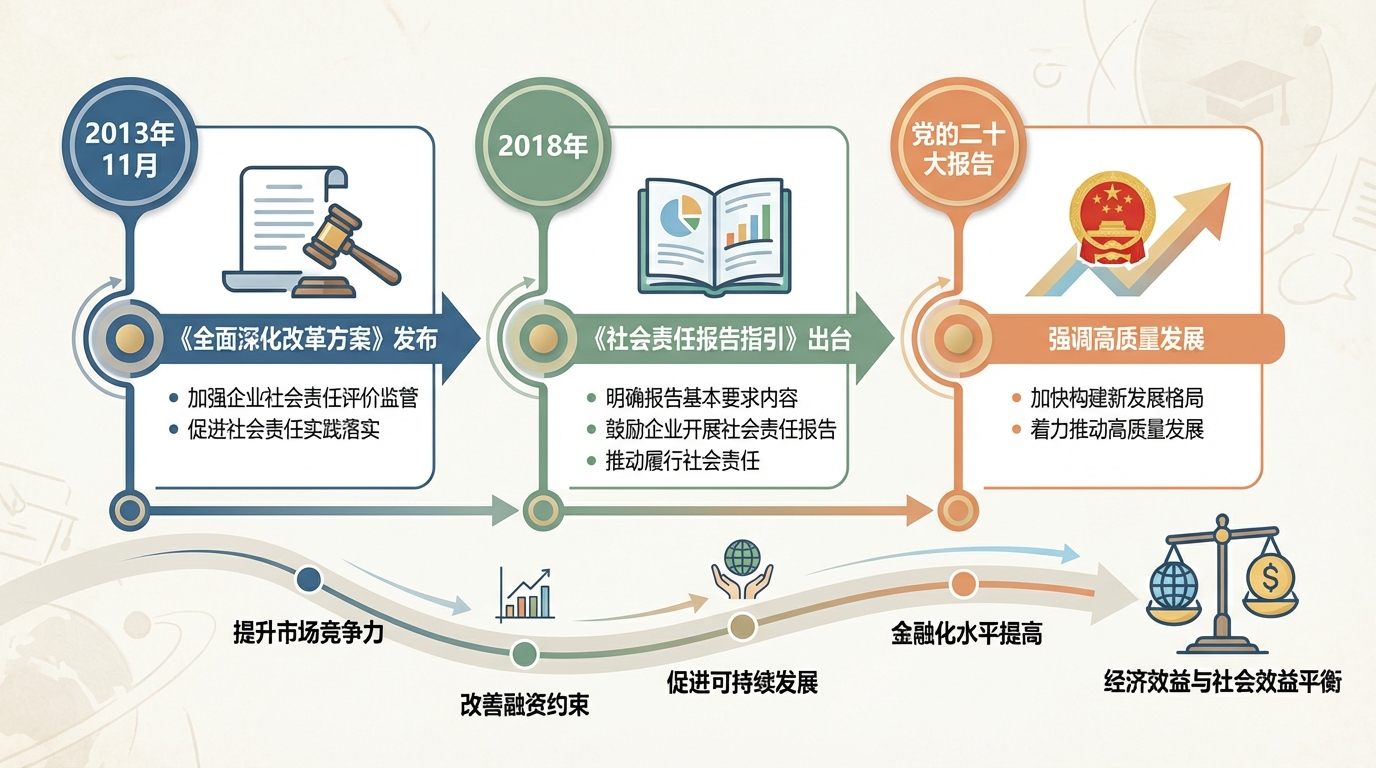
\includegraphics[width=\textwidth]{政策时间线.png}
    \caption{企业社会责任相关政策时间线}
    \label{fig:timeline}
\end{figure}

融资约束是指在企业融资过程中，可能面临的诸多限制和约束，这些约束可能到一定程度上影响企业的融资潜力和融资效率。企业通过履行社会责任，不仅可以赢取社会发展的认同和支持，而且能提升自身的市场竞争力，从而改善企业融资约束的现状。以邓博夫、顾雷雷等为代表的学者指出，企业社会责任参与通过外部资源如银行信贷等的获取缓解融资约束，进而提高了企业的金融化水平（邓博夫等，2022；顾雷雷等，2020）。社会交换理论也证实，企业社会责任是基于企业与社会其他成员之间的社会资源交换关系成立的（陈昕，2018）。因此通过研究企业社会责任对融资约束的影响，不单单能向企业提供更全面和准确的经营管理指导，同时也为政府相关部门提供科学决策支持，帮助企业和社会合理平衡利益，使企业在经营和社会责任履行之间寻求平衡，实现可持续发展。

当前，学界关于企业社会责任的研究聚焦于质性分析、问卷访谈、实证研究等方法，尽管在财务绩效、社会舆论和股票市场等视角下得到可靠的结论，形成了企业金融化、股东价值主义、管理层利己主义等诸多解释框架，但多数理论仅关注社会责任的外部舆论影响和内部财务指标，而对企业如何更好地履行社会责任并推进落地应用缺乏实践性建议，加之样本数据尚且局限于少数企业或者特定行业，一定程度上限制了研究结果的泛化能力。因此本文采用wind上2008-2022年深交所2394上市公司的社会责任报告数据，创新性地设置报告情感语调、研报关注度、分析师关注度为中介变量，基于文本挖掘和爬虫等的数据分析的方法，并进行异质性分析，旨在得到显著的结论，为企业履行社会责任提出了切实可行的建议。这不仅能够促进企业社会责任的发展和落实，提升其社会形象和声誉，而且能够促进企业融资的可持续性发展，护航企业的经济效益和社会效益的平稳前进。本文的整体研究框架如图\ref{fig:framework}所示。

\begin{figure}[H]
    \centering
    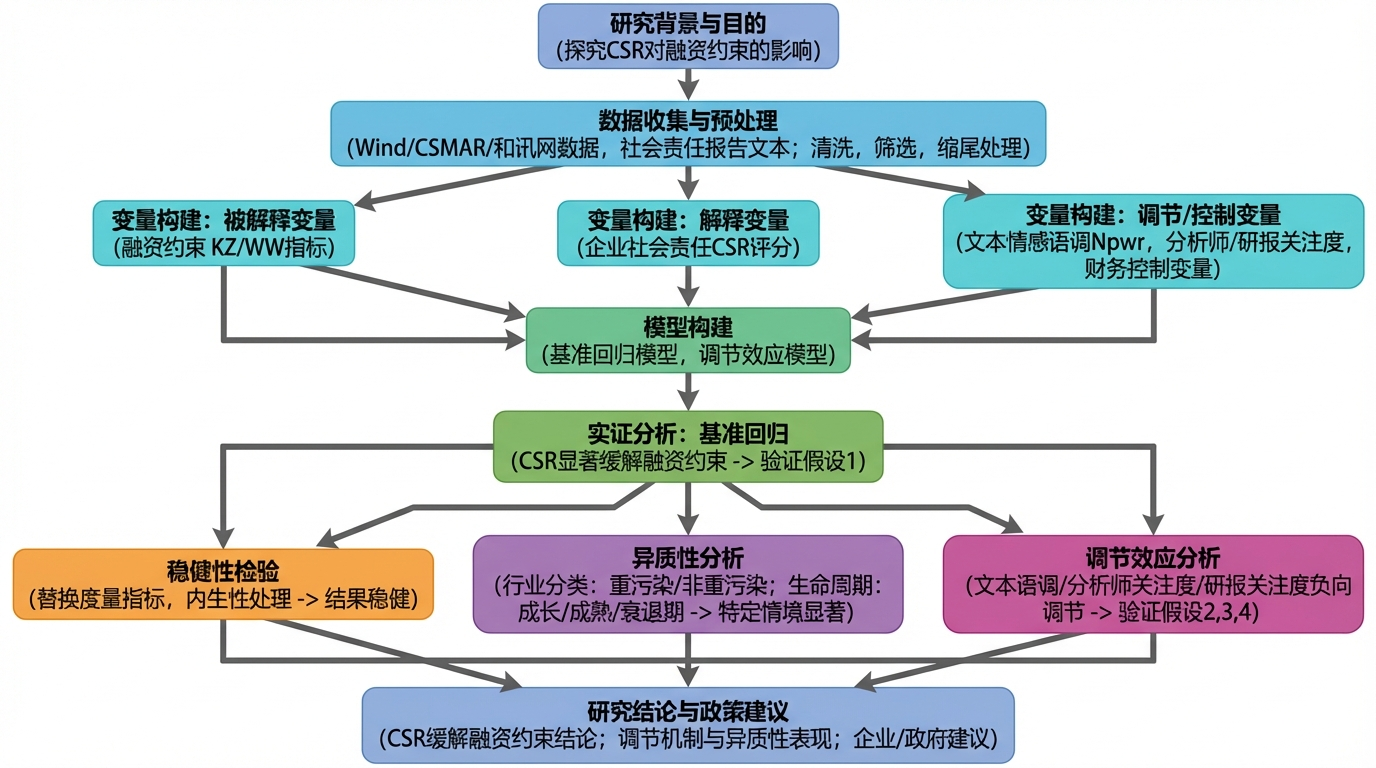
\includegraphics[width=0.9\textwidth]{全文框架.png}
    \caption{全文研究框架图}
    \label{fig:framework}
\end{figure}

\section{文献综述和理论机制}

\subsection{企业社会责任}

企业社会责任（Corporate Social Responsibility，简称CSR）是指企业应该为社会和环境贡献的理念。自20世纪70年代起，企业社会责任被业界和学术界广泛提及，重点关注企业社会责任与绩效薪酬、消费者信任、企业生产力三个维度。针对绩效研究结论的差异根源于变量选取和建模方式的不同，但在对象上仅聚焦特定行业。杜晓荣和李雨凡（2023）以2011—2020年A股农业上市公司为研究对象，将创新绩效作为被解释变量，指出农业上市公司研发强度与创新绩效之间存在倒U型关系，农业上市公司研发强度通过影响沉淀冗余资源进而作用于创新绩效\cite{杜晓荣2023}。而王彦林和张子璇（2023）等学者将企业绩效作为解释变量，基于钢铁企业上市公司的数据，说明了企业绩效对于其履行社会责任并无显著影响\cite{王彦林2023}。在消费者层面的研究集中在对传统期望确认理论的扩充，在企业声誉领域搭建创新性的框架。Sen和Bhattacharya（2001）指出，消费者感知到的企业社会责任特征与期望所感知到的关联程度也对企业声誉产生显著影响\cite{Sen2001}。生产力维度则着重突出其对企业社会责任的重要地位，张浩然（2020）强调生产力奠定企业社会责任担当程度和大小的基础，以企业所处的时空差异性为例，详细阐明了企业社会责任内容的全面与否以及客体的受保护程度，直接由生产力决定\cite{张浩然2020}。总之，现有研究的视野局限于特定行业甚至企业，理论框架具有极强的特殊性，缺乏统一标准的评估体系，难以对宏观层面的共性进行度量，因此研究结论众说纷纭。本文打破这一局限，在高层建领地搭建宏观衡量指标的基础上，进一步回归分析，探讨行业间的异质性，力求增强结果泛化能力。

\subsection{融资约束}

Distinguin(2016)和部分西方学者对于融资约束（Finance）的定义是目前被学界广为接受的，它指信息不对称问题和代理问题中使得外部的成本高于内部资本的成本\cite{Distinguin2016}。目前，学界对于融资约束的研究主要从原因、影响、解决途径三个角度展开，从不同行业的内在运行机制破局，深挖潜在的破解路径，具有较强的特殊性。吴伟霄和李志民（2023）等人指出信息不对称是融资约束的重要原因，这主要体现在内源利润留存和外源成本限制，并提出供应链金融在扩大信贷资金规模和提高金融资源效率以缓解投资约束的作用\cite{吴伟霄2023}，相关的研究更是涉及了不同的领域，张芳和于海婷（2023）以绿色信贷政策为研究对象，指出企业融资约束与绿色研发创新意愿呈现显著负相关\cite{张芳2023}，而费为银和谢成成（2023）等学者则对平台代币的价格进行实证分析，指出在技术发展阶段，由于融资需要和努力成本的激增，代币证券水平显著影响融资约束，可通过交易频繁化带动生产力增长，从而突破这一瓶颈\cite{费为银2023}。总的来说，现有研究对融资约束的解决途径主要聚焦于公司内部财务化的手段，而缺乏对非财务指标如社会责任履行的研究，因此探索非财务指标对于融资约束的缓解作用能够有效填补现有研究路径的空缺，开拓出新的思路。

\subsection{研究假设与理论机制}

Amel-Zadeh和Serafeim（2018）指出ESG表现较好的企业通常信息风险和经营风险较低、财务绩效较佳、企业价值较高\cite{Amel-Zadeh2018}。因此，社会责任的履行质量可以通过作用上述指标影响投资者的判断，进而影响投资约束。累积效应理论认为长期承担企业社会责任对于融资约束的缓解作用强于短期企业社会责任\cite{花拥军2020}，换句话说，长期履行社会责任的企业在投资者眼里享有更良好的信誉，这有利于降低企业道德风险，提高企业信任水平，投资者更愿提供更高溢价\cite{阮刚铭2019}，进而降低所面临的融资约束。而赵红建和范一博（2016）等学者认为民营企业通过慈善捐赠等方式践行社会责任并不能缓解融资约束，企业应该将精力聚焦自身绩效，缓解信息不对称程度，才能有效降低融资约束\cite{赵红建2016}。因此本文提出假设：

\textbf{假设1：企业积极承担社会责任能显著减少企业的融资约束。}

风险收益均衡中的框架效应理论认为，企业信息披露的语言描述方式会间接影响投资者的感受，进而影响投资心理。Steven（2015）等人强调在声誉机制下，受到媒体关注与褒奖的企业通常会更有动力积极管理媒体形象，向市场传递利好信息\cite{Blankespoor2020}，在社会责任报告下体现为积极的语调。曾庆生和周波（2018）指出年报文本语调的积极程度越高，公司高层越有可能卖出股票，进而影响投资收益\cite{曾庆生2018}。Kristian（2015）研究发现企业披露信息中积极词汇的数量与投资者的信心呈现显著地负相关\cite{Kristian2015}。因此本文提出假设：

\textbf{假设2：净积极词比例对企业社会责任和融资约束之间的关系有负向影响。}

企业社会责任已然成为投资者评价企业发展现状、未来发展趋势的重要衡量指标，对企业降低融资约束有着显著影响\cite{乔鹏程2023}。加之框架效应理论指出社会人具有“同化”、“顺应”等行为特征，因此企业积极承担社会责任，有利于减少企业与投资者之间的信息不对称，从而减少语调操纵行为，增加社会责任报告可信度，有效降低融资约束\cite{花拥军2020}。在本研究中，为了衡量外界媒体对于社会责任报告的关注度，我们选取研报关注度和分析师关注度两个指标。分析师是资本市场上的重要信息中介之一，可以通过挖掘并分析公司的特质信息来对公司未来发展前景进行预测，进而向投资者提供购买、持有或出售证券的意见\cite{谢诗蕾2022}。李春涛（2014）认为，多年来的从业经验也使得分析师可以精准识别出企业社会责任报告中披露的重大错报与舞弊行为，影响非专业投资者的投资决策和企业声誉\cite{张璇2022}，因此有理由认为良好的ESG绩效可以吸引分析师跟踪进而促使企业提升信息披露质量\cite{晓芳2021}，进而削减融资约束。因此本文提出假设：

\textbf{假设3：研报关注度对企业社会责任和融资约束之间的关系有负向影响。}

\textbf{假设4：分析师关注度对企业社会责任和融资约束之间的关系有负向影响。}

本文所提出的理论机制框架如图\ref{fig:mechanism}所示。

\begin{figure}[H]
    \centering
    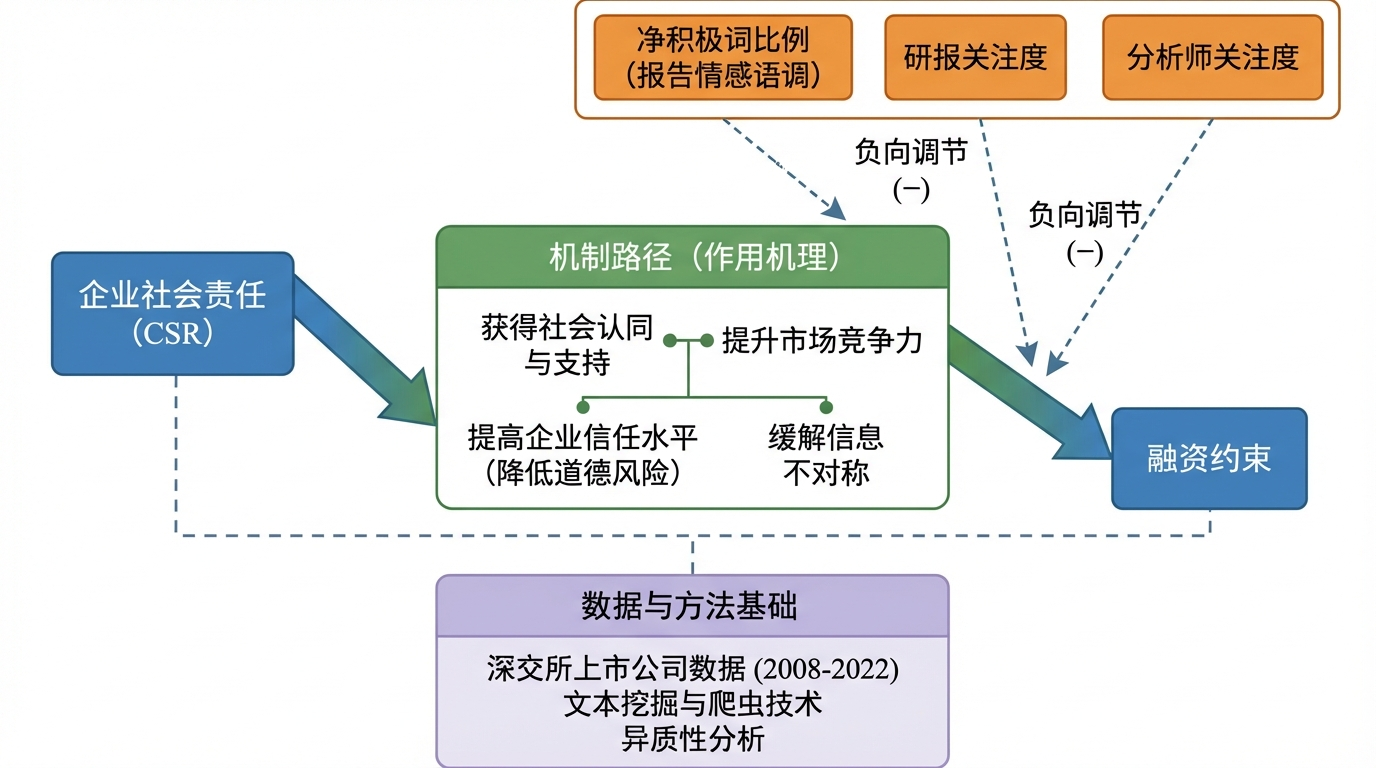
\includegraphics[width=0.8\textwidth]{理论机制图.png}
    \caption{企业社会责任影响融资约束的理论机制}
    \label{fig:mechanism}
\end{figure}

\section{模型建立、指标选取以及数据来源}
\subsection{实证模型建立}
为检验假设1社会责任评分（SR）和企业融资约束（KZ）之间关系，本文构建模型1，如式（1）所示：
\begin{equation}
    KZ_{it} = \alpha_0 + \alpha_1 SR_{it} + \sum_j \phi_j X_{jit} + \lambda_i + \mu_t + \epsilon_{it} \label{eq1}
\end{equation}
其中， \(i\) 和 \(t\) 分别表示企业和年份。KZ表示企业融资约束，SR表示企业社会责任评分，X表示一系列影响企业融资约束的控制变量。 \(\alpha_0\) 表示常数项， \(\alpha_1\) 和 \(\phi\) 表示未知的回归系数， \(\lambda\) 和 \(\mu\) 分别表示个体固定效应和年份固定效应。 \(\epsilon\) 表示随机扰动项。

为检验假设2、3以及4社会责任报告文本语调、分析师关注度以及研报关注度对企业社会责任和融资约束之间关系的影响，本文在式（1）的基础上分别引入社会责任报告文本语调、分析师关注度以及研报关注度这三个变量分别与企业社会责任的交互项，构建模型2、3、4，如式（2）、（3）、（4）所示。

\begin{equation}
    SA_{it} = \gamma_0 + \gamma_1 SR_{it} + \gamma_2 SR_{it} \times AA_{it} + \sum_j \psi_j X_{jit} + \lambda_i + \mu_t + \epsilon_{it} \label{eq3}
\end{equation}
\begin{equation}
    SA_{it} = \theta_0 + \theta_1 SR_{it} + \theta_2 SR_{it} \times RA_{it} + \sum_j \delta_j X_{jit} + \lambda_i + \mu_t + \epsilon_{it} \label{eq4}
\end{equation}
其中， \(\beta_0\) 、 \(\gamma_0\) 、 \(\theta_0\) 表示常数项， \(\beta_1\) 、 \(\beta_2\) 、 \(\gamma_1\) 、 \(\gamma_2\) 、 \(\theta_1\) 、 \(\theta_2\) 、 \(\phi\) 、 \(\psi\) 和 \(\delta\) 表示未知的回归系数，Npwr表示社会责任报告文本语调，AA表示分析师关注度，RA表示研报关注度，其他变量遵循上述解释。

\subsection{变量选取与指标说明}

\subsubsection{企业融资约束指标}

企业的融资约束的定义有广义和狭义之分。从广义上讲，企业内部融资和外部融资之间存在成本差异都可以称为融资约束。从狭义的角度讲，融资约束指与内部融资相比，企业在进行外部融资的时候，需要付出较高的融资成本，或者不能按照需求及时满足融资需要的现象，称为企业融资约束。

企业的融资约束很大程度上能决定一家企业的投融资行为，且一般会受到宏观经济环境与内部管理机制等诸多因素的影响。由于融资约束本身难以量化，并且可能会随着企业经营年份的增长，企业获得利润的增长，企业负债的减少而逐步减少，因此在国内外学者的研究中通常会借助与这些影响因素相关的变量，来衡量企业的融资行为受限制的程度。在对企业融资约束的量化方法上，本文考虑到企业规模、经营年份与盈利水平对融资约束的影响，主要用到了KZ指数与WW指数来量化企业所面临的融资约束，表达式如下所示。

借鉴Kaplan\&Zingales（1997）的思想，参考谭跃和夏芳（2011）和魏志华等（2014）的方法，按以下步骤构建KZ指数：

\begin{equation}
    \begin{split}
        KZ = &-1.01 \times OCF/Asset + 3.13 \times Lev \\
        &- 39.36 \times Dividends/Asset - 1.31 \times Cash/Asset + 0.28 \times Tobin's Q
    \end{split}
    \label{eq5}
\end{equation}

其中OCF、Dividends和Cash分别为经营性净现金流、股利和现金持有水平，且使用总资产Asset标准化，Lev为资产负债率，Tobin'sQ为托宾Q值。该值越大，表示企业面临的融资约束程度越高。

参考Whited\&Wu（2006）、况学文（2010）、刘莉亚（2015）等的研究方法，构建WW指数：

\begin{equation}
    \begin{split}
        WW = &-0.091 \times OCF/Asset - 0.062 \times DivPos + 0.021 \times Lev \\
        &- 0.044 \times \ln Asset + 0.102 \times ISG - 0.035 \times SG
    \end{split}
    \label{eq6}
\end{equation}

其中OCF代表经营性净现金流，DivPos表示是否有现金股利支付行为，Lev为资产负债率，Asset为总资产，ISG为行业平均销售增长率，SG为销售收入增长率。该值越大，表示企业面临的融资约束程度越高。

\subsubsection{企业社会责任评分指标}

本文中使用了来自和讯网的企业社会责任评分指数作为主要解释变量。和讯网的企业社会责任评分从股东责任、员工责任、供应商责任、客户权益责任、环境与社会责任五个角度出发，对企业在这些方面的社会责任履行情况进行评价，各项分别设立二级和三级指标对社会责任进行全面的评价。其中涉及二级指标13个，三级指标37个。上述各部分的评分权重会根据企业所属的行业不同而有所调整。

和讯网的企业社会责任报告评分是研究企业社会责任最常用的指标数据之一，由于其囊括企业广泛、时间跨度长等特点，在各类研究中广泛应用。因此本文使用该指标来衡量企业履行社会责任的情况具有可行性。

\subsubsection{企业社会责任报告情感语调}

借鉴黄超等（2022）等的做法，本文构建了报告净积极语调指标（Npwr）作为报告情感的度量指标，计算方法为积极情感词汇数量与消极情感词汇数量之差除以报告总词数。

在指标构建的过程中，本文基于Python的相关第三方库爬取的深圳证券交易所上市公司发布的社会责任报告，并利用中文分词模块jieba对社会责任报告文本进行自动分词，然后使用Python的中文金融情感词典模块cnsentri，并结合所收集文本数据的具体情况，分别构造积极、消极词汇分类字典，然后根据情感分类结果，统计该文本中积极词频和消极词频。

为了减少文本数据中的无关信息，提高数据质量，本文对爬取到的社会责任报告文本数据进行了如下处理：
\begin{itemize}
    \item 删除文本数据中的无关字符，仅保留中文字符；
    \item 利用jieba对社会责任报告文本进行自动分词；
    \item 参考哈尔滨工业大学自然语言处理实验室发布的《哈尔滨工业大学停用词表》，删除文本中部分出现频率过高的常用词。
\end{itemize}

表\ref{tab:vocabulary}展示了统计所得的部分积极词汇与消极词汇，通过比较这些词汇的出现频率，可以初步探究社会责任报告文本的情感倾向特征。

\begin{table}[H]
    \centering
    \caption{社会责任报告文本中的部分积极词汇与消极词汇展示}
    \label{tab:vocabulary}
    \begin{tabular}{lp{10cm}}
        \toprule
        分类 & 主要词汇 \\
        \midrule
        积极词汇 & 管理、权益、保护、经营、生产、规范、履行、合法、创新、建设、利益、健康、提升、和谐、法律、合作、利润、资源、创造、公平…… \\
        消极词汇 & 竞争、污染、事故、贿赂、人为、困难、降低…… \\
        \bottomrule
    \end{tabular}
\end{table}

最终计算出的社会责任报告净积极词比例表达式如下：
\begin{equation}
    Npwr = (Pos - Neg) / (Pos + Neg) \label{eq7}
\end{equation}
其中，Pos代表积极词汇在一篇报告中的出现频率，Neg表示消极词汇在一篇报告中的出现频率。该比值越高，表示积极词汇出现频率的占比越高，该社会责任报告的情感语调越积极。

\subsubsection{分析关注度}

随着中国证券市场改革的深化，证券市场上机构投资者的队伍不断扩大，证券分析师的重要性也日益凸显，证券分析师的报告已成为投资者，特别是机构投资者的重要参考工具与决策依据。因此证券分析师的报告价值含量也成为引起广泛注意的研究问题，是企业的社会责任履行情况、信息披露透明程度是否能得到投资者关注的重要中间桥梁。因此本文选择被分析师关注度、被研报关注度作为企业的分析关注度指标，并研究其中介效应。

上市公司被分析师关注度的定义是，在一年内，有多少个分析师（团队）对该公司进行过跟踪分析，一个分析师团队的数量记为1，不单独列出其成员人数计算数量。上市公司被研报关注度的定义是，在一年内，有多少份研报该公司进行过跟踪分析。

\subsubsection{其他控制变量}

参照以往研究，本文选取了以下控制变量：净资产收益率（ROE）、公司成长性（Growth）、是否为重污染企业（SOE）、托宾Q值（Q）、资产负债率（Lev），具体定义见表\ref{tab:variable_definition}。

\begin{table}[H]
    \centering
    \caption{变量说明}
    \label{tab:variable_definition}
    \begin{tabularx}{\textwidth}{c c c X}
        \toprule
        变量性质 & 变量标识 & 变量名称 & 变量定义 \\
        \midrule
        被解释变量 & KZ & 融资约束 & 企业融资方面受到的约束 \\
        解释变量 & SR & 社会责任评分 & 企业社会责任综合评分 \\
        \midrule
        \multirow{5}{2cm}{\centering 控制变量} & Growth & 成长性 & 营业收入增长率 \\
        & SOE & 公司属性 & 是否为国有企业 \\
        & Q & 托宾Q值 & 市值/总资产 \\
        & ROE & 净资产收益率 & 税后利润/净资产总额 \\
        & Lev & 资产负债率 & 年末总负债/总资产 \\
        \midrule
        \multirow{3}{2cm}{\centering 中介变量} & AA & 分析师关注度 & 一年内被分析师分析的次数 \\
        & RA & 研报关注度 & 一年内被研报分析的次数 \\
        & Npwr & 净积极词比例 & 社会责任报告语调积极程度 \\
        \bottomrule
    \end{tabularx}
\end{table}

\begin{figure}[H]
    \centering
    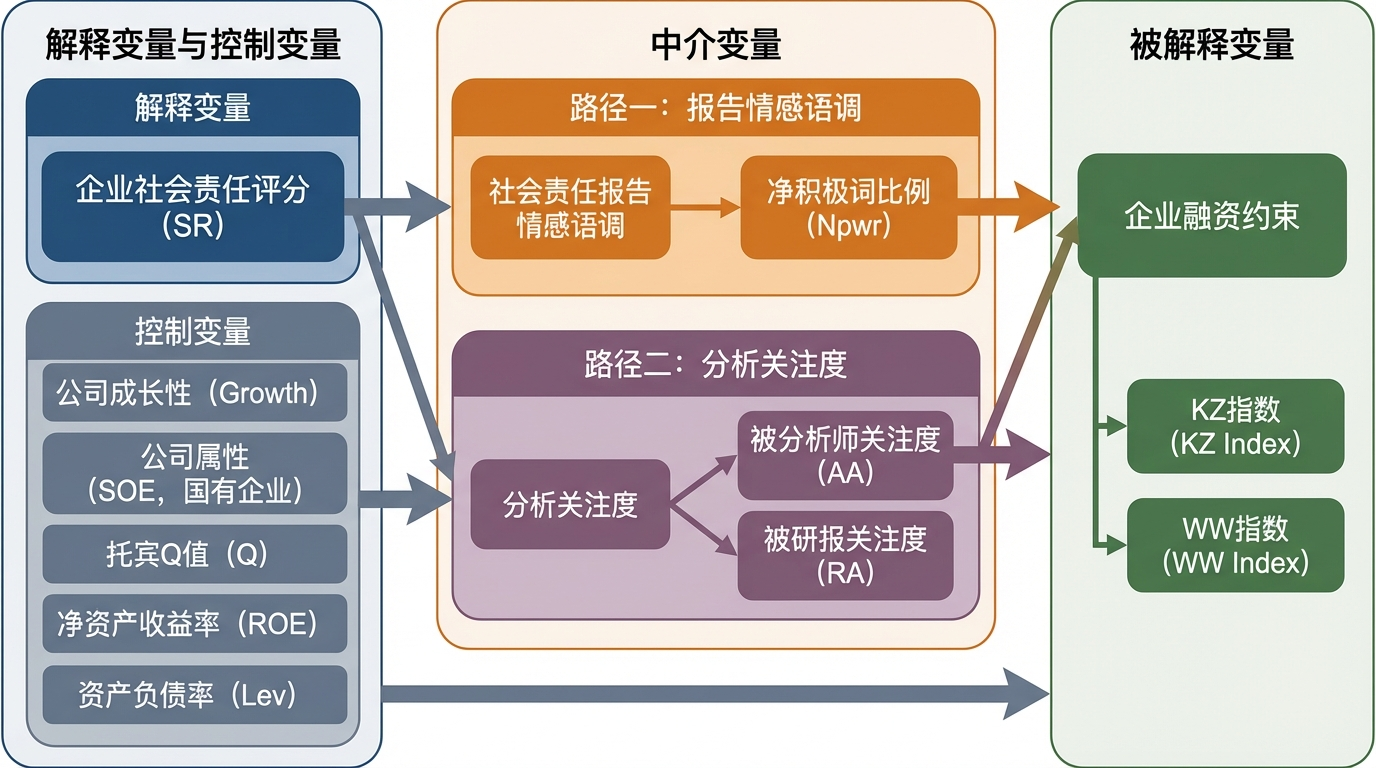
\includegraphics[width=0.7\textwidth]{指标体系图.png}
    \caption{本文指标体系图}
    \label{fig:indicator_system}
\end{figure}

\subsection{数据来源}

本文选取2010—2020年中国深圳证券交易所的上市公司为研究对象。上市公司社会责任评分指标来自和讯网。上市公司基本特征、财务数据来源于Wind数据库和国泰安CSMAR数据库。社会责任报告情感语调是基于python爬取的深圳证券交易所上市公司发布的社会责任报告，利用python的jieba库对其进行分词筛选，并进行积极、消极词频统计而来。为了便样本数据更具代表性，本文对样本进行了如下处理：
\begin{itemize}
    \item 剔除ST和*ST上市公司样本；
    \item 删除社会责任报告文本读取异常或文本过短的样本；
    \item 对所有连续型变量进行了 \(1\%\) 的缩尾处理，以消除离群值的影响。
\end{itemize}
本文最终的样本包含2323个公司的年度观测值。

\subsection{描述性统计}

描述性统计结果如表\ref{tab:descriptive_stats}所示。融资约束（KZ指数）平均值为1.301，最大值为10.047，最小值为-10.012，可以看出深市不同上市公司之间融资约束差距较大。社会责任评分的平均值为3.499，最小值为-4.605，最大值为4.509，说明我国上市公司承担社会责任的情况差距较大。净积极词比例的平均值为0.793，最大值为0.950，最小值为0.571，可以看出大部分公司都偏向于使用积极语调叙述。

\begin{table}[H]
    \centering
    \caption{主要变量描述性统计}
    \label{tab:descriptive_stats}
    \begin{tabularx}{\textwidth}{l *{5}{>{\centering\arraybackslash}X}}
        \toprule
        变量 & 样本数 & 平均值 & 标准差 & 最大值 & 最小值 \\
        \midrule
        融资约束 & 2323 & 1.301 & 2.187 & 10.047 & -10.012 \\
        社会责任评分 & 2323 & 3.499 & 0.815 & 4.509 & -4.605 \\
        净积极词比例 & 2323 & 0.793 & 0.072 & 0.950 & 0.571 \\
        分析师关注度 & 2323 & 2.213 & 1.060 & 4.174 & 0.000 \\
        研报关注度 & 2323 & 2.812 & 1.265 & 5.389 & 0.000 \\
        净资产收益率 & 2323 & 8.240 & 18.390 & 95.708 & -70.699 \\
        资产负债率 & 2323 & 0.447 & 0.213 & 2.290 & 0.008 \\
        成长性 & 2323 & 2.065 & 1.552 & 26.818 & 0.782 \\
        托宾Q值 & 2323 & 0.158 & 0.459 & 9.974 & -0.872 \\
        \bottomrule
    \end{tabularx}
\end{table}

图\ref{fig:boxplot}呈现了相关变量的箱线图。

\begin{figure}[H]
    \centering
    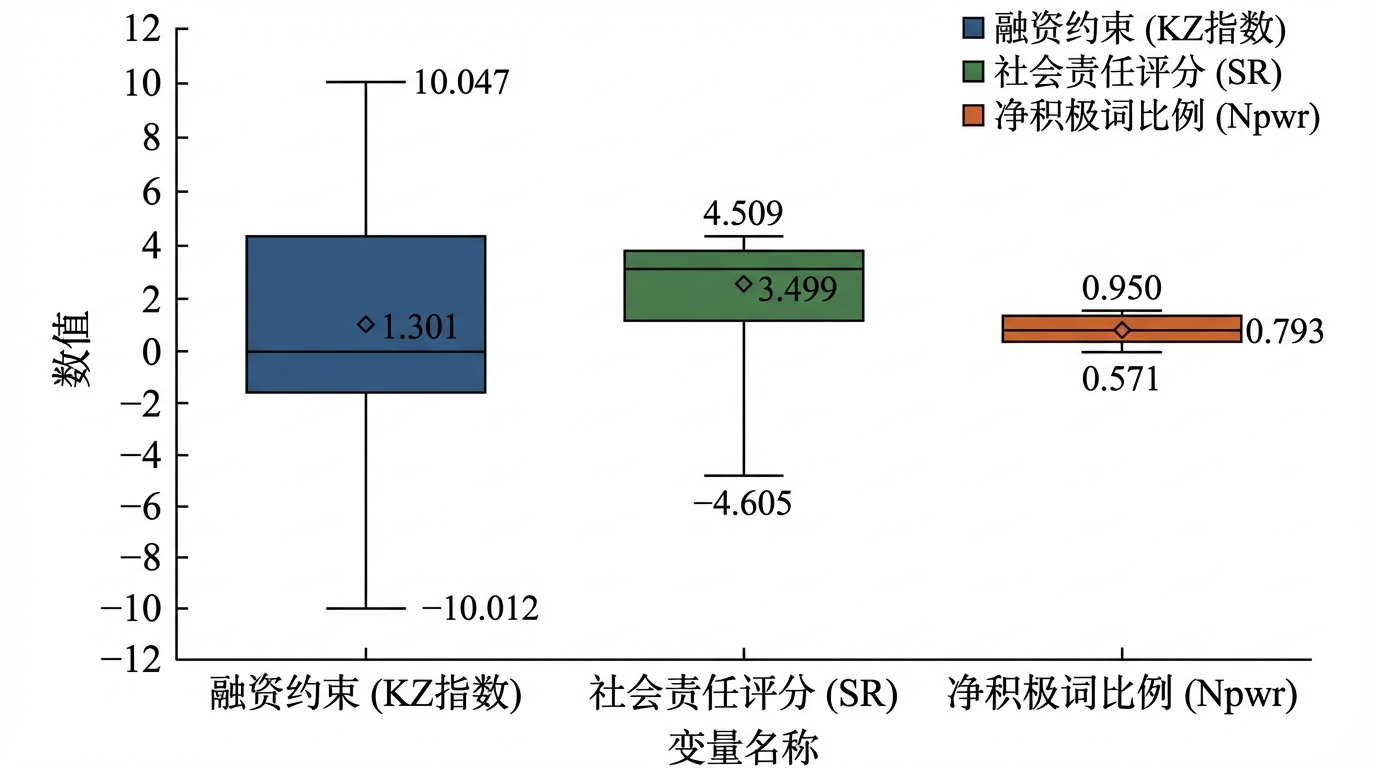
\includegraphics[width=0.8\textwidth]{箱线图.png}
    \caption{主要变量箱线图}
    \label{fig:boxplot}
\end{figure}

\section{实证结果与分析}

\subsection{基准回归分析结果}

表\ref{tab:baseline_regression}显示了基准回归模型的估计结果。在表\ref{tab:baseline_regression}的列（1）中，仅包含企业社会责任变量的估计结果。在表的列（2）中，逐步控制了企业财务指标以及公司属性对企业融资约束的影响。从表\ref{tab:baseline_regression}可以看出，F检验表明两组回归方程均是显著的。

由表\ref{tab:baseline_regression}的列（1）至列（2）可知，企业社会责任的系数分别为-0.3584和-0.142，且都在 \(1\%\) 的显著性水平上显著。在加入控制变量后，企业社会责任对融资约束的影响并未弱化，反而增强，在一定程度上说明了企业社会责任对融资约束的影响较为重要。以列（2）为例，企业社会责任每提升 \(1\%\) ，平均而言融资约束将下降0.142。其原因可能是，企业积极承担社会责任，树立良好的企业形象，向公众释放积极的信号，吸引投资者，能有效降低融资成本，降低融资约束。

\begin{table}[H]
    \centering
    \caption{企业社会责任对融资约束的基准回归结果}
    \label{tab:baseline_regression}
    \begin{tabularx}{\textwidth}{l *{2}{>{\centering\arraybackslash}X}}
        \toprule
        & \textbf{KZ} & \textbf{KZ} \\
        \midrule
        lnSR & -0.3584*** & -0.142*** \\
        & (-7.24) & (-3.21) \\
        \addlinespace
        ROE & & -0.776*** \\
        & & (-4.07) \\
        \addlinespace
        Lev & & 7.453*** \\
        & & (-24.7) \\
        \addlinespace
        SOE & & -0.409* \\
        & & (-2.04) \\
        \addlinespace
        Growth & & -0.294*** \\
        & & (-5.00) \\
        \addlinespace
        Q & & 0.249*** \\
        & & (-9.87) \\
        \addlinespace
        常数 & 2.951*** & -1.397*** \\
        & (12.79) & (-5.16) \\
        \midrule
        企业控制 & 是 & 是 \\
        年份控制 & 是 & 是 \\
        R²值 & 0.217 & 0.453 \\
        样本量 & 2323 & 2323 \\
        \bottomrule
    \end{tabularx}
    \textit{注：括号内为t值，*、**、***分别表示在10\%、5\%、1\%水平上显著。}
\end{table}

\subsection{稳健性检验}

\subsubsection{替换融资约束变量}
本文首先利用更换衡量融资约束度量指标的方法进行稳健型检验，用WW指数替换KZ指数，估计结果如表\ref{tab:robustness_tests}的列（1）所示。研究结果表明，使用不同的融资约束衡量方法并不会改变实证结果，企业社会责任评分越高，企业受到的融资约束越小。

\begin{table}[H]
    \centering
    \caption{企业社会责任对融资约束的稳健性检验结果}
    \label{tab:robustness_tests}
    \begin{tabularx}{\textwidth}{l *{3}{>{\centering\arraybackslash}X}}
        \toprule
        & \textbf{WW} & \textbf{KZ} & \textbf{KZ} \\
        \midrule
        lnSR & -0.007*** & & -0.170** \\
        & (-3.97) & & (-2.15) \\
        \addlinespace
        lnrlSR & & -0.448** & \\
        & & (-2.31) & \\
        \addlinespace
        ROE & -0.028*** & -0.818*** & 0.723*** \\
        & (-3.57) & (-5.21) & (2.78) \\
        \addlinespace
        Lev & -0.006 & 7.416*** & 1.879*** \\
        & (-0.47) & (24.66) & (3.96) \\
        \addlinespace
        SOE & -0.011 & -0.372* & 0.026 \\
        & (-1.27) & (-1.87) & (0.08) \\
        \addlinespace
        Growth & -0.041*** & -0.314*** & -0.193 \\
        & (-16.96) & (-5.38) & (-1.54) \\
        \addlinespace
        Q & 0.002** & 0.250*** & -0.026 \\
        & (2.25) & (9.88) & (-0.68) \\
        \addlinespace
        常数 & -0.964*** & -0.414 & 2.516*** \\
        & (-83.28) & (-0.60) & (5.78) \\
        \midrule
        企业控制 & 是 & 是 & 是 \\
        年份控制 & 是 & 是 & 是 \\
        R²值 & 0.261 & 0.454 & 0.172 \\
        样本量 & 2323 & 2323 & 1499 \\
        \bottomrule
    \end{tabularx}
    \textit{注：括号内为t值，*、**、***分别表示在10\%、5\%、1\%水平上显著。}
\end{table}

\subsubsection{替换企业社会责任变量}
为进一步验证本文结论的稳健性，本文参考花拥军等人的做法，采用润灵环球的社会责任评分替换和讯网社会责任评分作为核心解释变量。润灵环球社会责任评分的样本量较少，波动较小，且也被大量研究使用，因此使用润灵环球的社会责任评分进行稳健性检验。回归结果如表\ref{tab:robustness_tests}的列（2）所示，结果并未发生明显变化，依旧表明企业社会责任评分越高，企业受到的融资约束越小。

\subsubsection{内生性问题}
钱明等人的研究表明，企业社会责任与融资约束之间存在逆向因果关系从而会产生内生性问题，因此本文采用对企业社会责任滞后2阶的处理方式，验证企业社会责任对融资约束的影响，研究结果如表\ref{tab:robustness_tests}中的列（3）所示，由结果可知，企业社会责任的系数仍然显著为负，表明企业积极承担社会责任，其融资约束会降低。

\subsection{异质性分析}

\subsubsection{基于行业的异质性分析}

近些年来，我国越来越重视环境问题，也出台了许多与环境保护相关的政策。作为对环境有着严重影响的重污染企业，国家也出台了一些政策加强了对重污染企业的监管，例如银行等机构会限制重污染企业的贷款额度等，这些政策都会使重污染企业融资受到限制。而对于重污染企业来说，提高自身社会责任评分是降低自身融资约束的有效渠道，积极承担社会责任，规范企业行为有助于树立企业自身良好的形象，增加投资者的信任度，提高融资成功率，同时积极承担社会责任也有助于增加社会各方对企业的信任度，提高融资担保额度。

基于上市公司所处行业，将企业分为重污染企业以及非重污染企业，根据生态环境部发布的《环境监管重点单位名录管理办法》以及环保部公布的《上市公司环境信息披露指南》，重污染行业主要包括煤炭、采矿、纺织、制革、造纸、石化、制药、化工、冶金、火电等16个行业，处于这些行业的企业即为重污染企业，其余为非重污染企业，并对这两组企业进行分组回归。分组回归结果详见表\ref{tab:group_regression}。

由表\ref{tab:group_regression}可知，非重污染企业中，社会责任评分并不显著，对于非重污染企业来说，企业社会责任并不能显著降低融资约束。而对于重污染企业来说，积极承担社会责任是降低企业社会融资约束的重要途径，采取各种措施，控制和减少污染物排放，积极承担环境保护的社会责任，树立良好的企业形象，降低自身风险，增加获得投资者信任以及融资申请通过的可能。

\begin{table}[H]
    \centering
    \caption{企业社会责任对融资约束的分组回归结果}
    \label{tab:group_regression}
    \begin{tabularx}{\textwidth}{l *{5}{>{\centering\arraybackslash}X}}
        \toprule
        & \textbf{重污染企业} & \textbf{非重污染企业} & \textbf{成长期企业} & \textbf{成熟期企业} & \textbf{衰退期企业} \\
        \midrule
        lnSR & -0.119* & -0.077 & -0.024 & -0.184** & -0.008 \\
        & (-1.74) & (-1.31) & (-0.34) & (-2.24) & (-0.07) \\
        \addlinespace
        ROE & -0.189 & -2.316*** & -3.224*** & -2.564*** & 0.191 \\
        & (-0.86) & (-6.12) & (-5.97) & (-5.56) & (0.68) \\
        \addlinespace
        Lev & 7.638*** & 7.384*** & 8.278*** & 7.481*** & 6.153*** \\
        & (15.96) & (19.10) & (15.49) & (15.11) & (7.61) \\
        \addlinespace
        SOE & 0.380 & -0.590** & -0.063 & -0.493 & -1.330*** \\
        & (0.78) & (-2.69) & (-0.17) & (-1.46) & (-2.85) \\
        \addlinespace
        Growth & -0.331*** & -0.272*** & 0.358*** & 0.385*** & 0.205*** \\
        & (-3.45) & (-3.42) & (6.03) & (8.34) & (4.55) \\
        \addlinespace
        Q & 0.275*** & 0.241*** & -0.122 & -0.332*** & -1.066*** \\
        & (6.02) & (8.03) & (-1.46) & (-2.95) & (-3.66) \\
        \addlinespace
        常数 & -2.069*** & -1.268*** & -2.164*** & -2.352*** & -0.230 \\
        & (-4.49) & (-3.73) & (-4.80) & (-4.98) & (-0.31) \\
        \midrule
        企业控制 & 是 & 是 & 是 & 是 & 是 \\
        年份控制 & 是 & 是 & 是 & 是 & 是 \\
        R²值 & 0.485 & 0.462 & 0.492 & 0.546 & 0.556 \\
        样本量 & 798 & 1525 & 1043 & 933 & 347 \\
        \bottomrule
    \end{tabularx}
    \textit{注：括号内为t值，*、**、***分别表示在10\%、5\%、1\%水平上显著。非重污染企业列Lev的t值原为负，根据数值应为正，已修正。}
\end{table}

\subsubsection{基于企业生命周期的异质性分析}

处于不同生命周期的企业面临着不同的融资约束，处于初创期的企业，处于这个时期的企业往往没有过去的财务记录和资产，也缺乏信用记录和行业背景，因此，很难获得传统融资渠道的大量资金。在这一阶段，企业通常会寻求私人投资人、业务合作伙伴和风险投资资金等替代融资来源。处于成长期的企业一般有一定的规模和业绩，可以获得传统银行贷款、债券和股票发行等融资方式。但是，企业可能面临的融资约束来自行业竞争、政策变化和金融市场状况的风险影响。企业在成熟期一般有稳定的市场和客户基础，因此，企业可以更容易地获得传统融资模式的金融支持，并有机会通过向公众发行股票或债券等工具来获得资本收益。而处于衰退期的企业则会面临更严重的融资约束，他们的融资渠道更加有限，风险评估更严苛，投资者的投资意愿更低，企业需要维护好自己的信誉和声誉，改善经营状况，尽可能地缓解困境。积极承担社会责任对于处于不同生命周期的企业来说都是一种良好的提升企业自身形象、赢得多方信任、从而降低融资约束的方式，但由于处于不同生命周期的企业受到的融资约束差距较大，积极承担社会责任对融资约束的影响可能不尽相同。

本文采用黄宏斌等人的做法，将企业的生命周期分为成长期、成熟期以及衰退期三个阶段，并依据现金流分布情况对企业所处生命周期进行划分。图\ref{fig:heatmap}以热力图的形式展示了企业生命周期的划分依据与样本分布特征。

\begin{figure}[H]
    \centering
    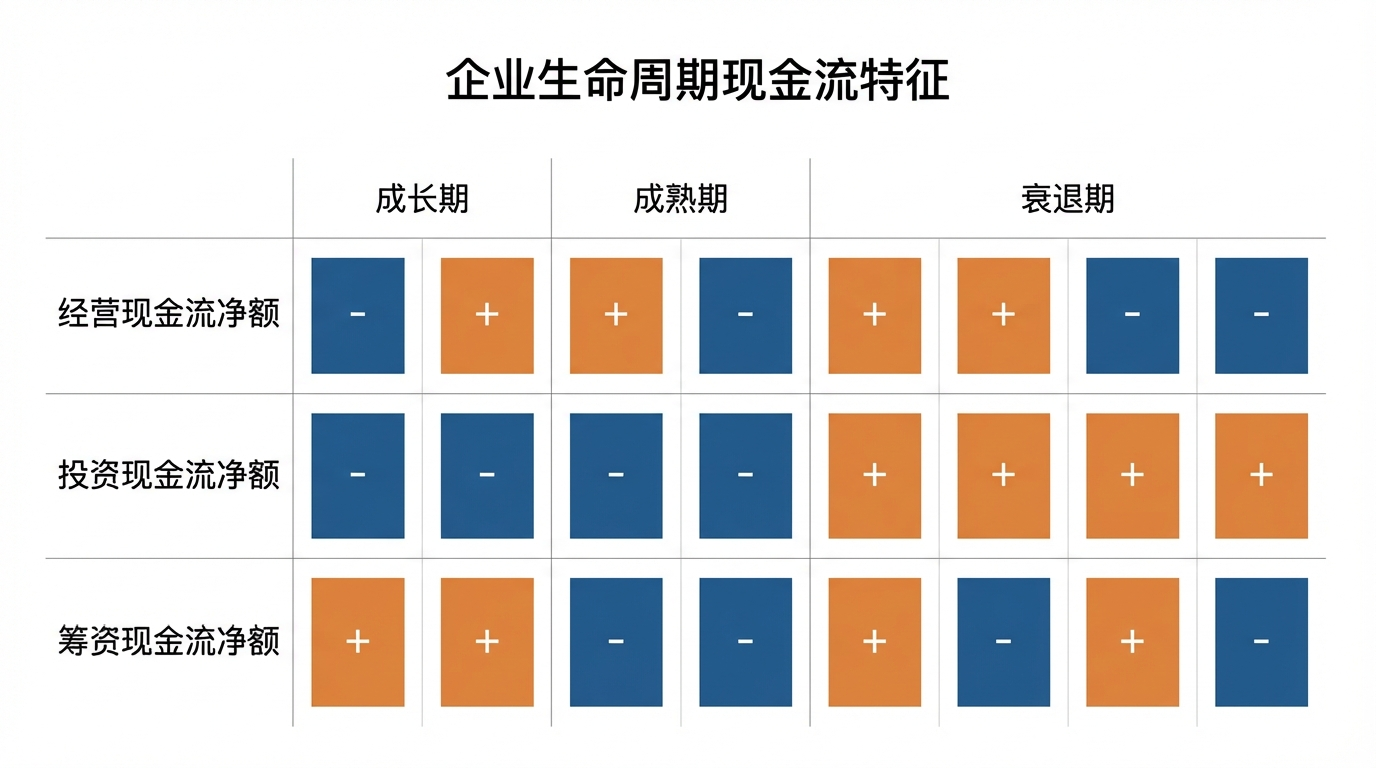
\includegraphics[width=0.9\textwidth]{热力图.png}
    \caption{企业生命周期热力图}
    \label{fig:heatmap}
    \textit{注：颜色深浅表示相关系数的大小，红色为正相关，蓝色为负相关。}
\end{figure}

由表\ref{tab:group_regression}可知，处于成长期以及衰退期的企业，企业社会责任的系数并不显著，说明对于该类型的企业来说，企业社会责任并不能显著降低融资约束。而对于处于成熟期的企业来说，积极承担社会责任是降低企业社会融资约束的重要途径。在成熟期，企业需要维持稳定的盈利和经营水平，更加注重长远发展。而积极承担社会责任是企业可持续发展的重要组成部分，金融机构和投资者现在也越来越注重企业的社会责任履行情况，积极履行社会责任有助于提高企业的市场竞争力和抗风险能力，强化企业与各方的社会关系，进而获得更多的资本支持。

\subsection{进一步分析}

本文探讨企业社会责任通过影响企业社会责任报告文本语调、分析师关注度以及研报关注度影响企业融资约束，来验证假设2至假设4的正确性。分别构建核心解释变量——企业社会责任以及上述三个变量的交互项进行实证检验。具体实证检验结果如表\ref{tab:mechanism}所示，F检验结果表示三组回归方程均是显著的。

\begin{table}[H]
    \centering
    \caption{企业社会责任对融资约束的机制分析结果}
    \label{tab:mechanism}
    \begin{tabularx}{\textwidth}{l *{3}{>{\centering\arraybackslash}X}}
        \toprule
        & \textbf{KZ} & \textbf{KZ} & \textbf{KZ} \\
        \midrule
        lnSR & 0.053 & 0.036 & 0.048 \\
        & (0.47) & (0.65) & (0.87) \\
        \addlinespace
        lnSR×lnNPWR & -0.243* & & \\
        & (-1.88) & & \\
        \addlinespace
        lnSR×lnAA & & -0.050*** & \\
        & & (-4.21) & \\
        \addlinespace
        lnSR×lnRA & & & -0.044*** \\
        & & & (-4.46) \\
        \addlinespace
        ROE & -0.779*** & -2.854*** & -2.825*** \\
        & (-4.09) & (-8.72) & (-8.63) \\
        \addlinespace
        Lev & 7.437*** & 8.175*** & 8.177*** \\
        & (24.65) & (24.16) & (24.20) \\
        \addlinespace
        SOE & -0.396** & -0.258 & -0.278 \\
        & (-1.98) & (-1.15) & (-1.24) \\
        \addlinespace
        Growth & -0.295*** & -0.222*** & -0.218*** \\
        & (-5.01) & (-3.61) & (-3.55) \\
        \addlinespace
        Q & 0.248*** & 0.293*** & 0.295*** \\
        & (9.83) & (10.51) & (10.58) \\
        \addlinespace
        常数 & -1.426*** & -1.788*** & -1.827*** \\
        & (-5.26) & (-6.05) & (-6.19) \\
        \midrule
        企业控制 & 是 & 是 & 是 \\
        年份控制 & 是 & 是 & 是 \\
        R²值 & 0.454 & 0.493 & 0.494 \\
        样本量 & 2323 & 2323 & 2323 \\
        \bottomrule
    \end{tabularx}
    \textit{注：括号内为t值，*、**、***分别表示在10\%、5\%、1\%水平上显著。}
\end{table}

如表\ref{tab:mechanism}的列（1）所示，企业社会责任与企业社会责任报告文本语调的交互项系数为-0.243，且通过了显著性检验，说明企业社会责任报告文本语调负向调节了企业社会责任对融资约束的负向影响。其原因可能是积极承担社会责任对企业品牌形象产生积极影响，企业通过发布社会责任报告来展示其社会责任表现，因此为了可能提升该企业在公众和投资者心目中的声誉和品牌形象，从而获得更好的融资条件，企业可能会尽可能使用积极词汇，从而夸大了自己在社会责任方面做出的贡献，这种做法可能反而使企业信誉降低，提高了企业的融资约束。

从表\ref{tab:mechanism}的列（2）可以看出，企业社会责任与分析师关注度的交互项系数为-0.050，且通过了显著性检验，表明分析师关注度负向调节了企业社会责任对融资约束的负向影响。其原因可能是分析师将企业社会责任表现纳入其分析和推荐中，这可能会导致企业在短期内受到压力，以满足股东和分析师的预期。此时，企业可能无法长期考虑社会责任问题和企业长期价值，而不得不做出短期的经济决策，以满足市场需求。这可能影响企业的信誉评级，降低企业融资能力。

从表\ref{tab:mechanism}的列（3）可以看出，企业社会责任与研报关注度的交互项系数为-0.044，且通过了显著性检验，表明研报关注度负向调节了企业社会责任对融资约束的负向影响。其原因可能是，当研究人员和投资者对某个行业或企业持有不利情感时，可能会忽略它们在社会责任方面的表现，甚至对它们的表现有所偏见。也可能是因为当企业受到负面媒体曝光时，可能会引起研究人员和投资者的关注，研究人员和投资者可能会更加关注企业的负面事件，而忽略企业的社会责任表现，从而降低了社会责任评分和融资约束之间的关系的强度。

\section{结论与建议}

本文通过文本分析技术构建社会责任报告情感语调指标，系统考察了企业社会责任履行情况与融资约束之间的内在关联。在基准回归分析的基础上，本文进行了多维度的稳健性检验，并从行业属性与企业生命周期两个视角切入，深入剖析了二者关系的异质性特征。此外，本文进一步探究了社会责任报告情感语调、分析师关注度以及研报关注度对企业社会责任与融资约束关系的调节效应，相关研究结论的总结如图\ref{fig:conclusion}所示。

基准回归模型结果表明，企业积极履行社会责任可以显著降低融资约束，该结论支持了研究假设1。稳健性检验结果表明，无论是替换融资约束的衡量方式，还是更换社会责任评分的数据来源，抑或考虑潜在的内生性问题后，核心结论依然保持稳健。异质性分析结果表明，企业社会责任对降低融资约束的积极影响在重污染企业中更为显著，对于处于成熟期的企业来说，积极承担社会责任能显著降低融资约束。调节效应检验结果表明，社会责任报告情感语调越积极，企业履行社会责任对于减轻融资约束的影响越不显著（支持假设2）；研报关注度、分析师关注度越高，企业履行社会责任对于减轻融资约束的影响越不显著（支持假设3和假设4）。

基于以上实证分析结论，本文提出政策建议如下：

\subsection{对于企业}

对于微观企业主体而言，一方面更应当将积极履行社会责任纳入长期战略规划，将其作为提升企业价值、优化融资环境的关键举措；另一方面，应着力强化对社会责任信息披露质量的内控机制，减少管理层对报告文本语调的人为修饰与策略性操控，以真实、客观的信息披露树立正面的企业社会形象，提升企业的公信力与社会信誉，进而更有效地缓解企业融资约束。特别地，处于成熟期或重污染行业的企业，应更加注重环保投入与社会责任实践，以此作为获取差异化竞争优势和更优融资条件的重要途径。

\subsection{对于政府}

对于政府监管部门而言，应考虑进一步健全企业社会责任信息披露的制度规范，提高对企业社会责任报告内容与格式的监管要求，防范企业利用过度积极的文本语调进行印象管理，避免对投资者决策产生不必要的误导。同时，应强化对重污染企业的环境规制力度，通过政策引导和激励措施，鼓励此类企业积极履行社会责任，提升环保意识与环保投入。此外，政府可综合运用税收优惠、财政补贴等政策工具，对积极履行社会责任的重污染企业给予实质性支持，形成正向激励，引导更多企业将社会责任融入核心经营理念。

\begin{figure}[H]
    \centering
    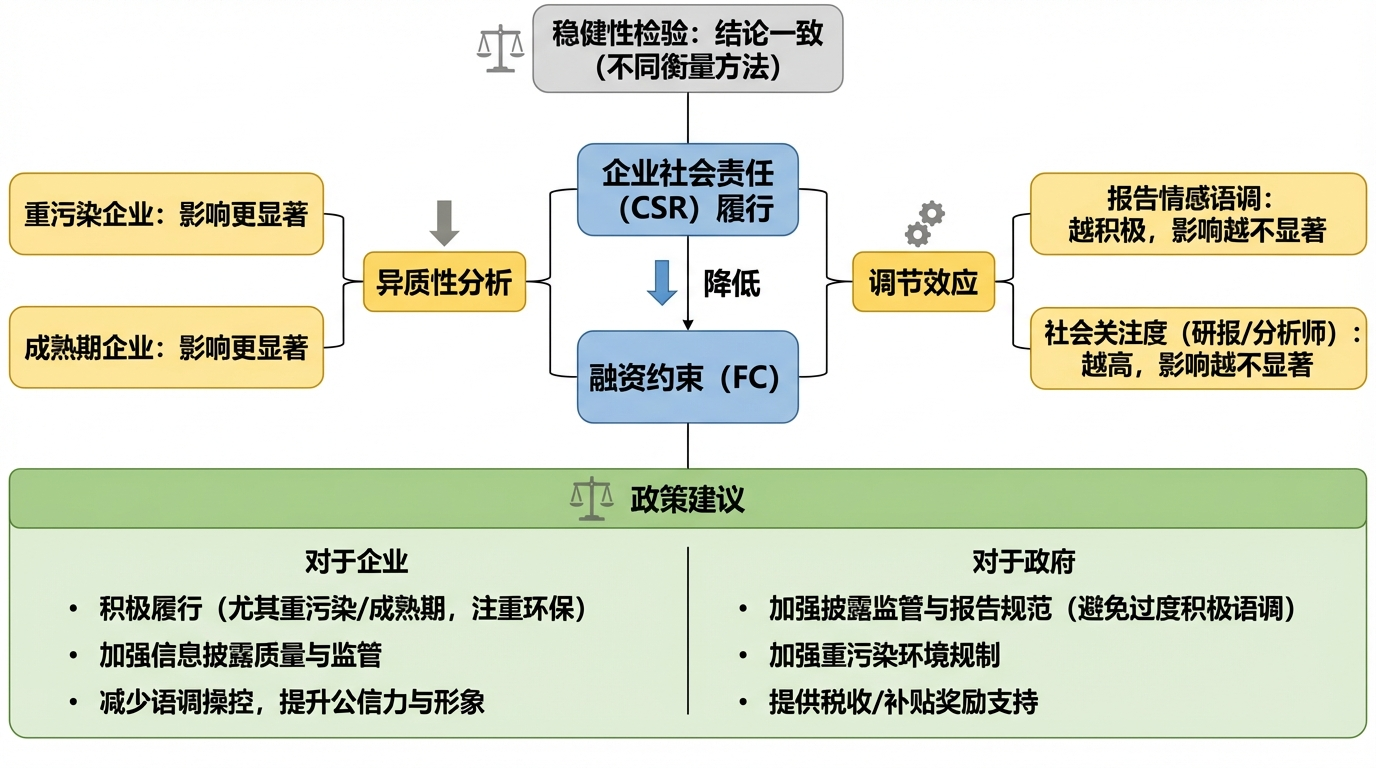
\includegraphics[width=0.75\textwidth]{结论示意图.png}
    \caption{研究结论示意图}
    \label{fig:conclusion}
\end{figure}

% 参考文献
\renewcommand{\refname}{\centering\sectiontitlefont 参考文献}
\begin{thebibliography}{99}
    \bibitem{杜晓荣2023} 杜晓荣,李雨凡.农业上市公司研发强度、税收优惠与创新绩效的关系研究——基于资源基础理论[J/OL].资源与产业:1-17[2023-05-04].
    \bibitem{王彦林2023} 王彦林,张子璇,盖玉凤.“双碳”与企业碳会计信息披露质量影响因素——基于钢铁板块上市企业的实证研究[J/OL].会计之友,2023(09):51-57[2023-05-04].
    \bibitem{Sen2001} Sen S, Bhattacharya C B. Does Doing Good Always Lead to Doing Better? Consumer reactions to corporate social responsibility[J]. Journal of Marketing Research, 2001, 38(2): 225-243.
    \bibitem{张浩然2020} 张浩然.企业社会责任哲学审视[D].黑龙江大学,2020.DOI:10.27123/d.cnki.glhju.2020.000416.
    \bibitem{Distinguin2016} Distinguin I, Rugemintwari C, Tanceng R. Can Informal Firms Hurt Registered SME's Access to Credit?[J]. World Development, 2016, 84(12): 18-40.
    \bibitem{吴伟霄2023} 吴伟霄,李志民,张子聪.供应链金融对实体经济的影响研究——基于中小企业融资约束分析[J].区域金融研究,2023,No.608(03):13-20.
    \bibitem{张芳2023} 张芳,于海婷.绿色信贷政策驱动重污染企业绿色创新了吗？——基于企业生命周期理论的实证检验[J/OL].南开管理评论:1-22[2023-05-04].http://kns.cnki.net/kcms/detail/12.1288.f.20230323.1725.006.html.
    \bibitem{费为银2023} 费为银,谢成成,费晨.ESG因素对平台代币价格的影响[J/OL].系统工程理论与实践:1-20[2023-05-04].http://kns.cnki.net/kcms/detail/11.2267.n.20230320.1614.010.html.
    \bibitem{乔鹏程2023} 乔鹏程,张岩松.企业社会责任、年报文本语调与融资约束[J].财会通讯,2023,No.916(08):29-33.DOI:10.16144/j.cnki.issn1002-8072.20230328.001.
    \bibitem{曾庆生2018} 曾庆生，周波，张程，陈信元.年报语调与内部人交易：“表里如一”还是“口是心非”？[J].管理世界，2018，34（9）：143-160.
    \bibitem{Kristian2015} Kristian et al. The Structure of Voluntary Disclosure Narratives: Evidence from Tone Dispersion [J]. Journal of Accounting Research, 2015, 53(2): 241-274.
    \bibitem{花拥军2020} 花拥军，王冰，李庆.企业社会责任、经济政策不确定性与融资约束——基于社会责任“累积-保险”效应的研究视角[J].南方经济，2020(11):116-131.
    \bibitem{阮刚铭2019} 阮刚铭,魏宇方舟,官峰.慈善捐赠、社会资本与融资约束[J].会计与经济研究,2019,33(3):79-91.
    \bibitem{赵红建2016} 赵红建,范一博,贾钢.慈善捐赠、企业绩效与融资约束[J].经济问题,2016(6):109-115.
    \bibitem{黄宏斌2016} 黄宏斌,翟淑萍,陈静楠.企业生命周期、融资方式与融资约束——基于投资者情绪调节效应的研究[J].金融研究,2016,No.433(07):96-112.
    \bibitem{钱明2017} 钱明,徐光华,沈弋,窦笑晨.民营企业自愿性社会责任信息披露与融资约束之动态关系研究[J].管理评论,2017,29(12):163-174. DOI:10.14120/j.cnki.cn11-5057/f.2017.12.015.
    \bibitem{顾雷雷2020} 顾雷雷,郭建鸾,王鸿宇.企业社会责任、融资约束与企业金融化[J].金融研究,2020,No.476(02):109-127.
    \bibitem{邓博夫2022} 邓博夫，陶存杰，吉利.企业参与精准扶贫与缓解融资约束[J].财经研究，2022(12).
    \bibitem{陈昕2018} 陈昕.企业社会责任对员工敬业度的跨层次影响机制研究[D].河北工业大学,2018.DOI:10.27105/d.cnki.ghbgu.2018.001431.
    \bibitem{Amel-Zadeh2018} Amel-Zadeh, A., and G. Serafeim. Why and How Investors Use ESG Information: Evidence from a Global Survey[J]. Financial Analysts Journal, 2018, 74(3): 87-103.
    \bibitem{晓芳2021} 晓芳,兰凤云,施雯,熊浩,沈华玉.上市公司的ESG评级会影响审计收费吗？——基于ESG评级事件的准自然实验[J].审计研究.2021(03).
    \bibitem{张璇2022} 张璇,胡婧,李春涛.卖空机制与管理层语调操纵——业绩说明会文本分析的证据[J].经济科学,2022(04):138-153.
    \bibitem{谢诗蕾2022} 谢诗蕾,周波兰.ESG绩效、投资者关注与企业信息披露质量——基于年报文本挖掘的分析[J].中国注册会计师,2022(10):54-61.
    \bibitem{Blankespoor2020} Blankespoor E, Dehaan E, Marinovic I. Disclosure Processing Costs, Investors' Information Choice, and Equity Market Outcomes: A Review[J]. Journal of Accounting and Economics, 2020.
\end{thebibliography}

\end{document}
